\documentclass[1p]{elsarticle_modified}
%\bibliographystyle{elsarticle-num}

%\usepackage[colorlinks]{hyperref}
%\usepackage{abbrmath_seonhwa} %\Abb, \Ascr, \Acal ,\Abf, \Afrak
\usepackage{amsfonts}
\usepackage{amssymb}
\usepackage{amsmath}
\usepackage{amsthm}
\usepackage{scalefnt}
\usepackage{amsbsy}
\usepackage{kotex}
\usepackage{caption}
\usepackage{subfig}
\usepackage{color}
\usepackage{graphicx}
\usepackage{xcolor} %% white, black, red, green, blue, cyan, magenta, yellow
\usepackage{float}
\usepackage{setspace}
\usepackage{hyperref}

\usepackage{tikz}
\usetikzlibrary{arrows}

\usepackage{multirow}
\usepackage{array} % fixed length table
\usepackage{hhline}

%%%%%%%%%%%%%%%%%%%%%
\makeatletter
\renewcommand*\env@matrix[1][\arraystretch]{%
	\edef\arraystretch{#1}%
	\hskip -\arraycolsep
	\let\@ifnextchar\new@ifnextchar
	\array{*\c@MaxMatrixCols c}}
\makeatother %https://tex.stackexchange.com/questions/14071/how-can-i-increase-the-line-spacing-in-a-matrix
%%%%%%%%%%%%%%%

\usepackage[normalem]{ulem}

\newcommand{\msout}[1]{\ifmmode\text{\sout{\ensuremath{#1}}}\else\sout{#1}\fi}
%SOURCE: \msout is \stkout macro in https://tex.stackexchange.com/questions/20609/strikeout-in-math-mode

\newcommand{\cancel}[1]{
	\ifmmode
	{\color{red}\msout{#1}}
	\else
	{\color{red}\sout{#1}}
	\fi
}

\newcommand{\add}[1]{
	{\color{blue}\uwave{#1}}
}

\newcommand{\replace}[2]{
	\ifmmode
	{\color{red}\msout{#1}}{\color{blue}\uwave{#2}}
	\else
	{\color{red}\sout{#1}}{\color{blue}\uwave{#2}}
	\fi
}

\newcommand{\Sol}{\mathcal{S}} %segment
\newcommand{\D}{D} %diagram
\newcommand{\A}{\mathcal{A}} %arc


%%%%%%%%%%%%%%%%%%%%%%%%%%%%%5 test

\def\sl{\operatorname{\textup{SL}}(2,\Cbb)}
\def\psl{\operatorname{\textup{PSL}}(2,\Cbb)}
\def\quan{\mkern 1mu \triangleright \mkern 1mu}

\theoremstyle{definition}
\newtheorem{thm}{Theorem}[section]
\newtheorem{prop}[thm]{Proposition}
\newtheorem{lem}[thm]{Lemma}
\newtheorem{ques}[thm]{Question}
\newtheorem{cor}[thm]{Corollary}
\newtheorem{defn}[thm]{Definition}
\newtheorem{exam}[thm]{Example}
\newtheorem{rmk}[thm]{Remark}
\newtheorem{alg}[thm]{Algorithm}

\newcommand{\I}{\sqrt{-1}}
\begin{document}

%\begin{frontmatter}
%
%\title{Boundary parabolic representations of knots up to 8 crossings}
%
%%% Group authors per affiliation:
%\author{Yunhi Cho} 
%\address{Department of Mathematics, University of Seoul, Seoul, Korea}
%\ead{yhcho@uos.ac.kr}
%
%
%\author{Seonhwa Kim} %\fnref{s_kim}}
%\address{Center for Geometry and Physics, Institute for Basic Science, Pohang, 37673, Korea}
%\ead{ryeona17@ibs.re.kr}
%
%\author{Hyuk Kim}
%\address{Department of Mathematical Sciences, Seoul National University, Seoul 08826, Korea}
%\ead{hyukkim@snu.ac.kr}
%
%\author{Seokbeom Yoon}
%\address{Department of Mathematical Sciences, Seoul National University, Seoul, 08826,  Korea}
%\ead{sbyoon15@snu.ac.kr}
%
%\begin{abstract}
%We find all boundary parabolic representation of knots up to 8 crossings.
%
%\end{abstract}
%\begin{keyword}
%    \MSC[2010] 57M25 
%\end{keyword}
%
%\end{frontmatter}

%\linenumbers
%\tableofcontents
%
\newcommand\colored[1]{\textcolor{white}{\rule[-0.35ex]{0.8em}{1.4ex}}\kern-0.8em\color{red} #1}%
%\newcommand\colored[1]{\textcolor{white}{ #1}\kern-2.17ex	\textcolor{white}{ #1}\kern-1.81ex	\textcolor{white}{ #1}\kern-2.15ex\color{red}#1	}

{\Large $\underline{11a_{60}~(K11a_{60})}$}

\setlength{\tabcolsep}{10pt}
\renewcommand{\arraystretch}{1.6}
\vspace{1cm}\begin{tabular}{m{100pt}>{\centering\arraybackslash}m{274pt}}
\multirow{5}{120pt}{
	\centering
	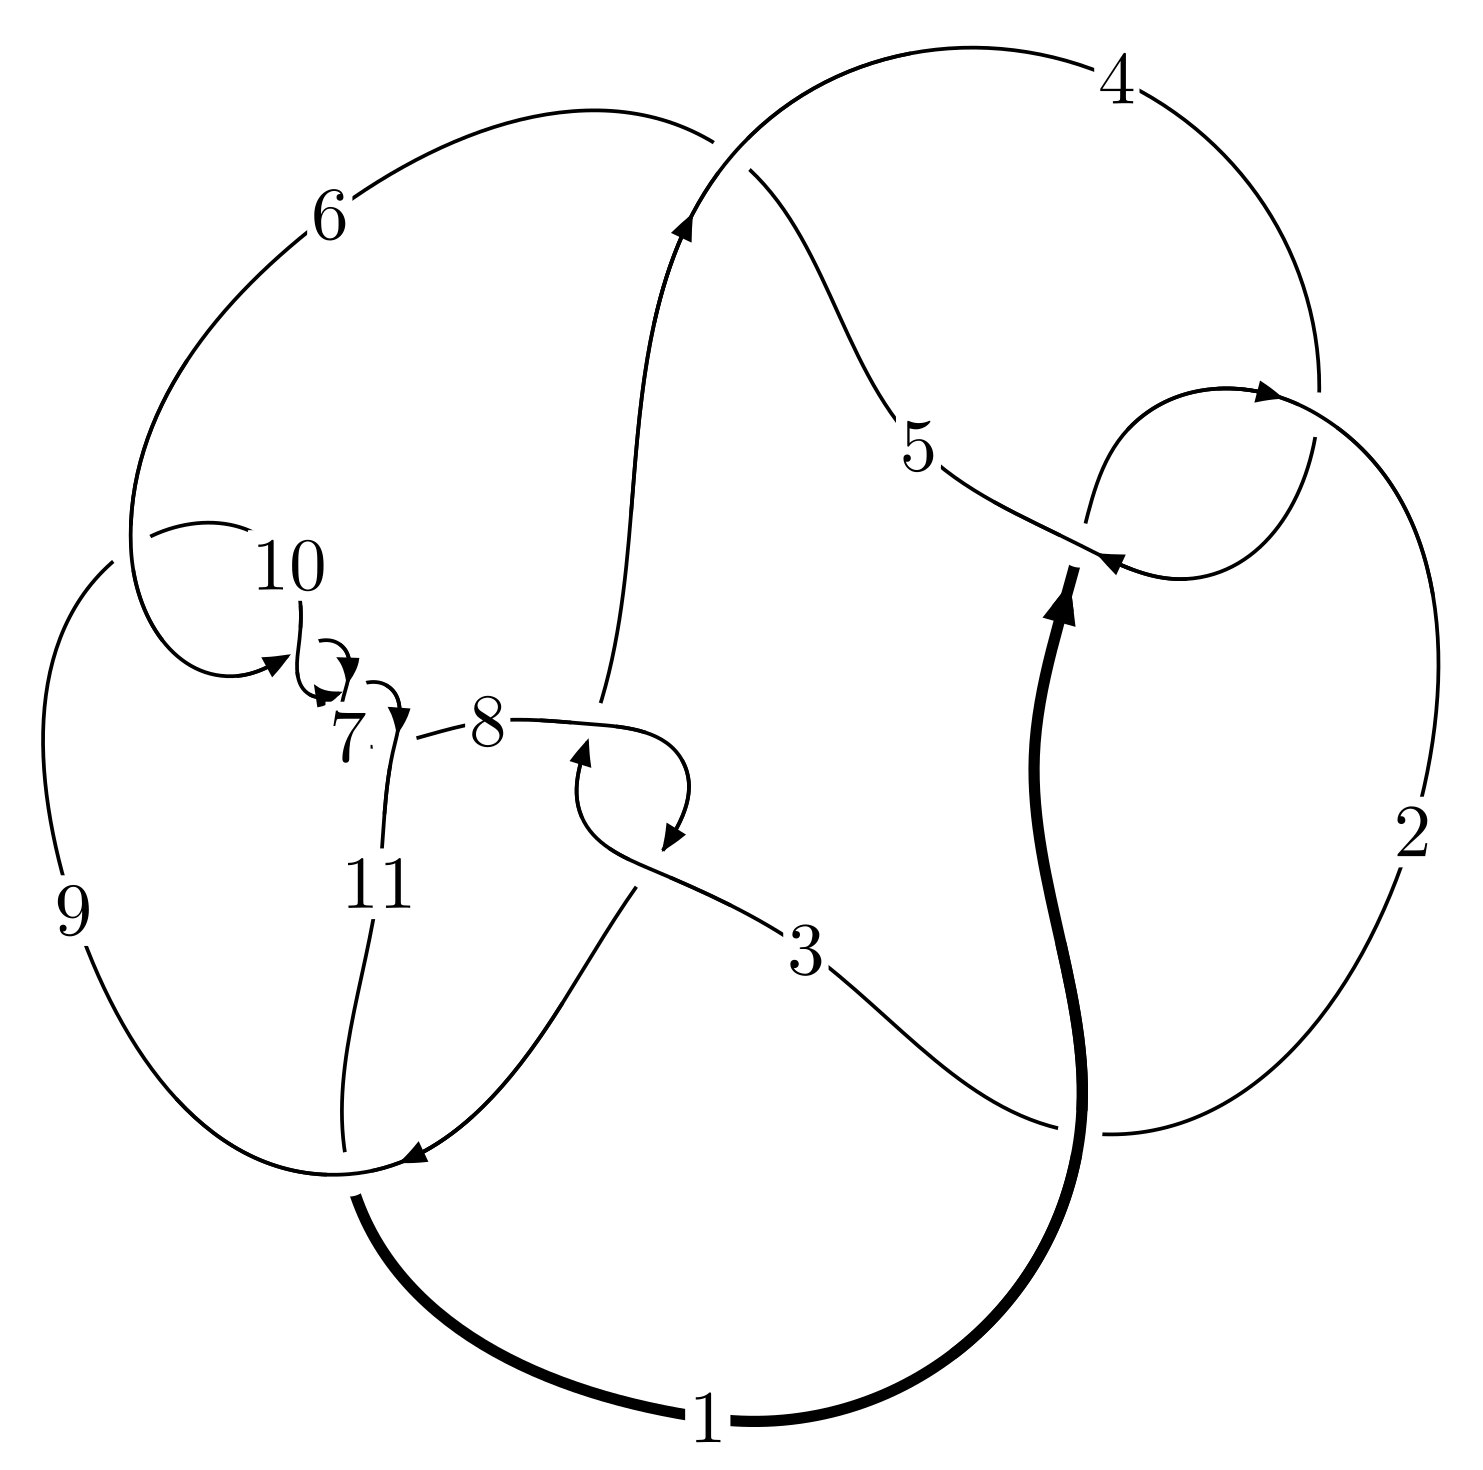
\includegraphics[width=112pt]{../../../GIT/diagram.site/Diagrams/png/309_11a_60.png}\\
\ \ \ A knot diagram\footnotemark}&
\allowdisplaybreaks
\textbf{Linearized knot diagam} \\
\cline{2-2}
 &
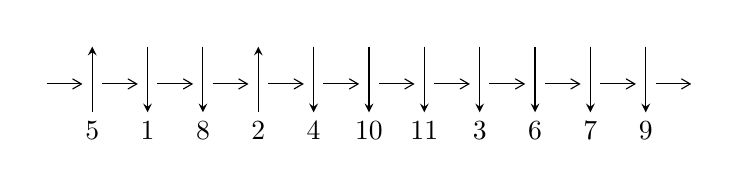
\begin{tikzpicture}[x=20pt, y=17pt]
	% nodes
	\node (C0) at (0, 0) {};
	\node (C1) at (1, 0) {};
	\node (C1U) at (1, +1) {};
	\node (C1D) at (1, -1) {5};

	\node (C2) at (2, 0) {};
	\node (C2U) at (2, +1) {};
	\node (C2D) at (2, -1) {1};

	\node (C3) at (3, 0) {};
	\node (C3U) at (3, +1) {};
	\node (C3D) at (3, -1) {8};

	\node (C4) at (4, 0) {};
	\node (C4U) at (4, +1) {};
	\node (C4D) at (4, -1) {2};

	\node (C5) at (5, 0) {};
	\node (C5U) at (5, +1) {};
	\node (C5D) at (5, -1) {4};

	\node (C6) at (6, 0) {};
	\node (C6U) at (6, +1) {};
	\node (C6D) at (6, -1) {10};

	\node (C7) at (7, 0) {};
	\node (C7U) at (7, +1) {};
	\node (C7D) at (7, -1) {11};

	\node (C8) at (8, 0) {};
	\node (C8U) at (8, +1) {};
	\node (C8D) at (8, -1) {3};

	\node (C9) at (9, 0) {};
	\node (C9U) at (9, +1) {};
	\node (C9D) at (9, -1) {6};

	\node (C10) at (10, 0) {};
	\node (C10U) at (10, +1) {};
	\node (C10D) at (10, -1) {7};

	\node (C11) at (11, 0) {};
	\node (C11U) at (11, +1) {};
	\node (C11D) at (11, -1) {9};
	\node (C12) at (12, 0) {};

	% arrows
	\draw[->,>={angle 60}]
	(C0) edge (C1) (C1) edge (C2) (C2) edge (C3) (C3) edge (C4) (C4) edge (C5) (C5) edge (C6) (C6) edge (C7) (C7) edge (C8) (C8) edge (C9) (C9) edge (C10) (C10) edge (C11) (C11) edge (C12) ;	\draw[->,>=stealth]
	(C1D) edge (C1U) (C2U) edge (C2D) (C3U) edge (C3D) (C4D) edge (C4U) (C5U) edge (C5D) (C6U) edge (C6D) (C7U) edge (C7D) (C8U) edge (C8D) (C9U) edge (C9D) (C10U) edge (C10D) (C11U) edge (C11D) ;
	\end{tikzpicture} \\
\hhline{~~} \\& 
\textbf{Solving Sequence} \\ \cline{2-2} 
 &
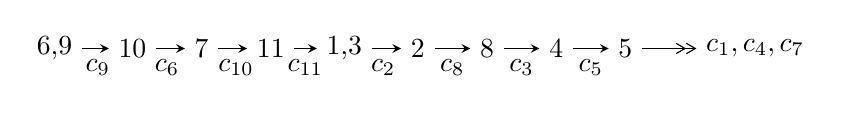
\begin{tikzpicture}[x=25pt, y=7pt]
	% node
	\node (A0) at (-1/8, 0) {6,9};
	\node (A1) at (1, 0) {10};
	\node (A2) at (2, 0) {7};
	\node (A3) at (3, 0) {11};
	\node (A4) at (65/16, 0) {1,3};
	\node (A5) at (41/8, 0) {2};
	\node (A6) at (49/8, 0) {8};
	\node (A7) at (57/8, 0) {4};
	\node (A8) at (65/8, 0) {5};
	\node (C1) at (1/2, -1) {$c_{9}$};
	\node (C2) at (3/2, -1) {$c_{6}$};
	\node (C3) at (5/2, -1) {$c_{10}$};
	\node (C4) at (7/2, -1) {$c_{11}$};
	\node (C5) at (37/8, -1) {$c_{2}$};
	\node (C6) at (45/8, -1) {$c_{8}$};
	\node (C7) at (53/8, -1) {$c_{3}$};
	\node (C8) at (61/8, -1) {$c_{5}$};
	\node (A9) at (10, 0) {$c_{1},c_{4},c_{7}$};

	% edge
	\draw[->,>=stealth]	
	(A0) edge (A1) (A1) edge (A2) (A2) edge (A3) (A3) edge (A4) (A4) edge (A5) (A5) edge (A6) (A6) edge (A7) (A7) edge (A8) ;
	\draw[->>,>={angle 60}]	
	(A8) edge (A9);
\end{tikzpicture} \\ 

\end{tabular} \\

\footnotetext{
The image of knot diagram is generated by the software ``\textbf{Draw programme}" developed by Andrew Bartholomew(\url{http://www.layer8.co.uk/maths/draw/index.htm\#Running-draw}), where we modified some parts for our purpose(\url{https://github.com/CATsTAILs/LinksPainter}).
}\phantom \\ \newline 
\centering \textbf{Ideals for irreducible components\footnotemark of $X_{\text{par}}$} 
 
\begin{align*}
I^u_{1}&=\langle 
- u^{44}- u^{43}+\cdots+3 u^2+b,\;-8 u^{45}-5 u^{44}+\cdots+2 a+11,\;u^{46}+3 u^{45}+\cdots+3 u-1\rangle \\
I^u_{2}&=\langle 
b,\;a^2- a u+a- u+2,\;u^2- u-1\rangle \\
\\
\end{align*}
\raggedright * 2 irreducible components of $\dim_{\mathbb{C}}=0$, with total 50 representations.\\
\footnotetext{All coefficients of polynomials are rational numbers. But the coefficients are sometimes approximated in decimal forms when there is not enough margin.}
\newpage
\renewcommand{\arraystretch}{1}
\centering \section*{I. $I^u_{1}= \langle - u^{44}- u^{43}+\cdots+3 u^2+b,\;-8 u^{45}-5 u^{44}+\cdots+2 a+11,\;u^{46}+3 u^{45}+\cdots+3 u-1 \rangle$}
\flushleft \textbf{(i) Arc colorings}\\
\begin{tabular}{m{7pt} m{180pt} m{7pt} m{180pt} }
\flushright $a_{6}=$&$\begin{pmatrix}0\\u\end{pmatrix}$ \\
\flushright $a_{9}=$&$\begin{pmatrix}1\\0\end{pmatrix}$ \\
\flushright $a_{10}=$&$\begin{pmatrix}1\\u^2\end{pmatrix}$ \\
\flushright $a_{7}=$&$\begin{pmatrix}- u\\- u^3+u\end{pmatrix}$ \\
\flushright $a_{11}=$&$\begin{pmatrix}- u^2+1\\- u^4+2 u^2\end{pmatrix}$ \\
\flushright $a_{1}=$&$\begin{pmatrix}u^4-3 u^2+1\\- u^4+2 u^2\end{pmatrix}$ \\
\flushright $a_{3}=$&$\begin{pmatrix}4 u^{45}+\frac{5}{2} u^{44}+\cdots+18 u-\frac{11}{2}\\u^{44}+u^{43}+\cdots-7 u^3-3 u^2\end{pmatrix}$ \\
\flushright $a_{2}=$&$\begin{pmatrix}2 u^{45}+\frac{1}{2} u^{44}+\cdots+12 u-\frac{7}{2}\\-\frac{3}{2} u^{45}-\frac{3}{2} u^{44}+\cdots-\frac{9}{2} u+\frac{3}{2}\end{pmatrix}$ \\
\flushright $a_{8}=$&$\begin{pmatrix}u^3-2 u\\u^5-3 u^3+u\end{pmatrix}$ \\
\flushright $a_{4}=$&$\begin{pmatrix}u^{45}-\frac{1}{2} u^{44}+\cdots+11 u-\frac{7}{2}\\-5 u^{45}-7 u^{44}+\cdots-14 u+4\end{pmatrix}$ \\
\flushright $a_{5}=$&$\begin{pmatrix}\frac{1}{2} u^{44}+u^{43}+\cdots-5 u-\frac{1}{2}\\- u^{14}+8 u^{12}+\cdots+u^2+2 u\end{pmatrix}$\\ \flushright $a_{5}=$&$\begin{pmatrix}\frac{1}{2} u^{44}+u^{43}+\cdots-5 u-\frac{1}{2}\\- u^{14}+8 u^{12}+\cdots+u^2+2 u\end{pmatrix}$\\&\end{tabular}
\flushleft \textbf{(ii) Obstruction class $= -1$}\\~\\
\flushleft \textbf{(iii) Cusp Shapes $= -\frac{21}{2} u^{45}-16 u^{44}+\cdots-\frac{31}{2} u+3$}\\~\\
\newpage\renewcommand{\arraystretch}{1}
\flushleft \textbf{(iv) u-Polynomials at the component}\newline \\
\begin{tabular}{m{50pt}|m{274pt}}
Crossings & \hspace{64pt}u-Polynomials at each crossing \\
\hline $$\begin{aligned}c_{1},c_{4}\end{aligned}$$&$\begin{aligned}
&u^{46}+3 u^{45}+\cdots+7 u+1
\end{aligned}$\\
\hline $$\begin{aligned}c_{2},c_{5}\end{aligned}$$&$\begin{aligned}
&u^{46}+15 u^{45}+\cdots-45 u+1
\end{aligned}$\\
\hline $$\begin{aligned}c_{3},c_{8}\end{aligned}$$&$\begin{aligned}
&u^{46}+u^{45}+\cdots-48 u-16
\end{aligned}$\\
\hline $$\begin{aligned}c_{6},c_{7},c_{9}\\c_{10}\end{aligned}$$&$\begin{aligned}
&u^{46}+3 u^{45}+\cdots+3 u-1
\end{aligned}$\\
\hline $$\begin{aligned}c_{11}\end{aligned}$$&$\begin{aligned}
&u^{46}-11 u^{45}+\cdots+5 u-73
\end{aligned}$\\
\hline
\end{tabular}\\~\\
\newpage\renewcommand{\arraystretch}{1}
\flushleft \textbf{(v) Riley Polynomials at the component}\newline \\
\begin{tabular}{m{50pt}|m{274pt}}
Crossings & \hspace{64pt}Riley Polynomials at each crossing \\
\hline $$\begin{aligned}c_{1},c_{4}\end{aligned}$$&$\begin{aligned}
&y^{46}+15 y^{45}+\cdots-45 y+1
\end{aligned}$\\
\hline $$\begin{aligned}c_{2},c_{5}\end{aligned}$$&$\begin{aligned}
&y^{46}+35 y^{45}+\cdots-2249 y+1
\end{aligned}$\\
\hline $$\begin{aligned}c_{3},c_{8}\end{aligned}$$&$\begin{aligned}
&y^{46}+25 y^{45}+\cdots+2176 y+256
\end{aligned}$\\
\hline $$\begin{aligned}c_{6},c_{7},c_{9}\\c_{10}\end{aligned}$$&$\begin{aligned}
&y^{46}-53 y^{45}+\cdots-9 y+1
\end{aligned}$\\
\hline $$\begin{aligned}c_{11}\end{aligned}$$&$\begin{aligned}
&y^{46}+7 y^{45}+\cdots+31219 y+5329
\end{aligned}$\\
\hline
\end{tabular}\\~\\
\newpage\flushleft \textbf{(vi) Complex Volumes and Cusp Shapes}
$$\begin{array}{c|c|c}  
\text{Solutions to }I^u_{1}& \I (\text{vol} + \sqrt{-1}CS) & \text{Cusp shape}\\
 \hline 
\begin{aligned}
u &= \phantom{-}0.683033 + 0.585511 I \\
a &= -1.17131 + 1.61239 I \\
b &= -0.586768 - 1.279220 I\end{aligned}
 & \phantom{-}4.58631 - 10.20080 I & -5.76564 + 8.71859 I \\ \hline\begin{aligned}
u &= \phantom{-}0.683033 - 0.585511 I \\
a &= -1.17131 - 1.61239 I \\
b &= -0.586768 + 1.279220 I\end{aligned}
 & \phantom{-}4.58631 + 10.20080 I & -5.76564 - 8.71859 I \\ \hline\begin{aligned}
u &= -1.107400 + 0.146429 I \\
a &= \phantom{-}0.192350 + 0.087991 I \\
b &= -0.167779 - 1.185070 I\end{aligned}
 & \phantom{-}1.38563 - 2.89669 I & -7.00000 + 0. I\phantom{ +0.000000I} \\ \hline\begin{aligned}
u &= -1.107400 - 0.146429 I \\
a &= \phantom{-}0.192350 - 0.087991 I \\
b &= -0.167779 + 1.185070 I\end{aligned}
 & \phantom{-}1.38563 + 2.89669 I & -7.00000 + 0. I\phantom{ +0.000000I} \\ \hline\begin{aligned}
u &= \phantom{-}0.644087 + 0.591749 I \\
a &= \phantom{-}1.12925 - 1.65187 I \\
b &= \phantom{-}0.490901 + 1.297460 I\end{aligned}
 & \phantom{-}5.48925 - 4.23240 I & -3.97125 + 3.86585 I \\ \hline\begin{aligned}
u &= \phantom{-}0.644087 - 0.591749 I \\
a &= \phantom{-}1.12925 + 1.65187 I \\
b &= \phantom{-}0.490901 - 1.297460 I\end{aligned}
 & \phantom{-}5.48925 + 4.23240 I & -3.97125 - 3.86585 I \\ \hline\begin{aligned}
u &= -0.721560 + 0.271962 I \\
a &= \phantom{-}0.078758 - 0.314563 I \\
b &= -0.586991 - 0.576410 I\end{aligned}
 & -2.76000 + 0.49175 I & -14.4049 - 1.3153 I \\ \hline\begin{aligned}
u &= -0.721560 - 0.271962 I \\
a &= \phantom{-}0.078758 + 0.314563 I \\
b &= -0.586991 + 0.576410 I\end{aligned}
 & -2.76000 - 0.49175 I & -14.4049 + 1.3153 I \\ \hline\begin{aligned}
u &= \phantom{-}0.625541 + 0.443656 I \\
a &= -1.32103 + 1.86857 I \\
b &= -0.437369 - 0.962184 I\end{aligned}
 & -1.57427 - 4.58885 I & -10.12217 + 8.09100 I \\ \hline\begin{aligned}
u &= \phantom{-}0.625541 - 0.443656 I \\
a &= -1.32103 - 1.86857 I \\
b &= -0.437369 + 0.962184 I\end{aligned}
 & -1.57427 + 4.58885 I & -10.12217 - 8.09100 I\\
 \hline 
 \end{array}$$\newpage$$\begin{array}{c|c|c}  
\text{Solutions to }I^u_{1}& \I (\text{vol} + \sqrt{-1}CS) & \text{Cusp shape}\\
 \hline 
\begin{aligned}
u &= \phantom{-}0.307520 + 0.663659 I \\
a &= \phantom{-}0.67086 - 1.68681 I \\
b &= -0.327075 + 1.311180 I\end{aligned}
 & \phantom{-}6.48322 + 0.00049 I & -1.75811 + 1.98241 I \\ \hline\begin{aligned}
u &= \phantom{-}0.307520 - 0.663659 I \\
a &= \phantom{-}0.67086 + 1.68681 I \\
b &= -0.327075 - 1.311180 I\end{aligned}
 & \phantom{-}6.48322 - 0.00049 I & -1.75811 - 1.98241 I \\ \hline\begin{aligned}
u &= \phantom{-}0.259302 + 0.676556 I \\
a &= -0.61524 + 1.65084 I \\
b &= \phantom{-}0.443673 - 1.290370 I\end{aligned}
 & \phantom{-}5.83960 + 5.95442 I & -2.89350 - 3.47222 I \\ \hline\begin{aligned}
u &= \phantom{-}0.259302 - 0.676556 I \\
a &= -0.61524 - 1.65084 I \\
b &= \phantom{-}0.443673 + 1.290370 I\end{aligned}
 & \phantom{-}5.83960 - 5.95442 I & -2.89350 + 3.47222 I \\ \hline\begin{aligned}
u &= -1.280730 + 0.112519 I \\
a &= -0.245265 - 0.380738 I \\
b &= \phantom{-}0.020723 + 1.301980 I\end{aligned}
 & \phantom{-}1.51797 + 2.92543 I & \phantom{-0.000000 } 0 \\ \hline\begin{aligned}
u &= -1.280730 - 0.112519 I \\
a &= -0.245265 + 0.380738 I \\
b &= \phantom{-}0.020723 - 1.301980 I\end{aligned}
 & \phantom{-}1.51797 - 2.92543 I & \phantom{-0.000000 } 0 \\ \hline\begin{aligned}
u &= -0.529027 + 0.472674 I \\
a &= \phantom{-}0.104077 - 0.663139 I \\
b &= -1.023760 - 0.238308 I\end{aligned}
 & \phantom{-}1.28884 + 4.36080 I & -6.58604 - 6.72191 I \\ \hline\begin{aligned}
u &= -0.529027 - 0.472674 I \\
a &= \phantom{-}0.104077 + 0.663139 I \\
b &= -1.023760 + 0.238308 I\end{aligned}
 & \phantom{-}1.28884 - 4.36080 I & -6.58604 + 6.72191 I \\ \hline\begin{aligned}
u &= \phantom{-}0.480914 + 0.492416 I \\
a &= \phantom{-}0.97784 - 1.95842 I \\
b &= \phantom{-}0.137372 + 1.054990 I\end{aligned}
 & \phantom{-}2.15360 - 1.72767 I & -2.05511 + 4.46443 I \\ \hline\begin{aligned}
u &= \phantom{-}0.480914 - 0.492416 I \\
a &= \phantom{-}0.97784 + 1.95842 I \\
b &= \phantom{-}0.137372 - 1.054990 I\end{aligned}
 & \phantom{-}2.15360 + 1.72767 I & -2.05511 - 4.46443 I\\
 \hline 
 \end{array}$$\newpage$$\begin{array}{c|c|c}  
\text{Solutions to }I^u_{1}& \I (\text{vol} + \sqrt{-1}CS) & \text{Cusp shape}\\
 \hline 
\begin{aligned}
u &= -0.438186 + 0.463380 I \\
a &= -0.026707 + 0.771502 I \\
b &= \phantom{-}0.986397 + 0.062419 I\end{aligned}
 & \phantom{-}1.56190 - 1.05001 I & -5.35085 - 0.93346 I \\ \hline\begin{aligned}
u &= -0.438186 - 0.463380 I \\
a &= -0.026707 - 0.771502 I \\
b &= \phantom{-}0.986397 - 0.062419 I\end{aligned}
 & \phantom{-}1.56190 + 1.05001 I & -5.35085 + 0.93346 I \\ \hline\begin{aligned}
u &= -0.507626\phantom{ +0.000000I} \\
a &= \phantom{-}0.299451\phantom{ +0.000000I} \\
b &= \phantom{-}0.385891\phantom{ +0.000000I}\end{aligned}
 & -0.763627\phantom{ +0.000000I} & -13.0210\phantom{ +0.000000I} \\ \hline\begin{aligned}
u &= \phantom{-}1.52489 + 0.10717 I \\
a &= -0.593194 + 0.302209 I \\
b &= -1.107570 + 0.332603 I\end{aligned}
 & -5.01225 - 0.84578 I & \phantom{-0.000000 } 0 \\ \hline\begin{aligned}
u &= \phantom{-}1.52489 - 0.10717 I \\
a &= -0.593194 - 0.302209 I \\
b &= -1.107570 - 0.332603 I\end{aligned}
 & -5.01225 + 0.84578 I & \phantom{-0.000000 } 0 \\ \hline\begin{aligned}
u &= -1.52977 + 0.12312 I \\
a &= -0.863933 - 0.983761 I \\
b &= -0.377563 + 1.143250 I\end{aligned}
 & -4.55511 + 3.84471 I & \phantom{-0.000000 } 0 \\ \hline\begin{aligned}
u &= -1.52977 - 0.12312 I \\
a &= -0.863933 + 0.983761 I \\
b &= -0.377563 - 1.143250 I\end{aligned}
 & -4.55511 - 3.84471 I & \phantom{-0.000000 } 0 \\ \hline\begin{aligned}
u &= -1.53985 + 0.07420 I \\
a &= \phantom{-}0.78183 + 1.34401 I \\
b &= \phantom{-}0.289274 - 0.982056 I\end{aligned}
 & -7.15725 - 0.57650 I & \phantom{-0.000000 } 0 \\ \hline\begin{aligned}
u &= -1.53985 - 0.07420 I \\
a &= \phantom{-}0.78183 - 1.34401 I \\
b &= \phantom{-}0.289274 + 0.982056 I\end{aligned}
 & -7.15725 + 0.57650 I & \phantom{-0.000000 } 0 \\ \hline\begin{aligned}
u &= \phantom{-}1.54840 + 0.12785 I \\
a &= \phantom{-}0.555669 - 0.368908 I \\
b &= \phantom{-}1.123810 - 0.444850 I\end{aligned}
 & -5.69586 - 6.48224 I & \phantom{-0.000000 } 0\\
 \hline 
 \end{array}$$\newpage$$\begin{array}{c|c|c}  
\text{Solutions to }I^u_{1}& \I (\text{vol} + \sqrt{-1}CS) & \text{Cusp shape}\\
 \hline 
\begin{aligned}
u &= \phantom{-}1.54840 - 0.12785 I \\
a &= \phantom{-}0.555669 + 0.368908 I \\
b &= \phantom{-}1.123810 + 0.444850 I\end{aligned}
 & -5.69586 + 6.48224 I & \phantom{-0.000000 } 0 \\ \hline\begin{aligned}
u &= \phantom{-}1.56614\phantom{ +0.000000I} \\
a &= -0.397337\phantom{ +0.000000I} \\
b &= -0.732082\phantom{ +0.000000I}\end{aligned}
 & -7.96363\phantom{ +0.000000I} & \phantom{-0.000000 } 0 \\ \hline\begin{aligned}
u &= \phantom{-}0.374900 + 0.216095 I \\
a &= -0.66143 + 2.89217 I \\
b &= -0.016090 - 0.601274 I\end{aligned}
 & -0.45061 + 1.71194 I & -2.49876 + 0.88608 I \\ \hline\begin{aligned}
u &= \phantom{-}0.374900 - 0.216095 I \\
a &= -0.66143 - 2.89217 I \\
b &= -0.016090 + 0.601274 I\end{aligned}
 & -0.45061 - 1.71194 I & -2.49876 - 0.88608 I \\ \hline\begin{aligned}
u &= -1.57913 + 0.12981 I \\
a &= \phantom{-}1.16947 + 0.97231 I \\
b &= \phantom{-}0.561226 - 1.073100 I\end{aligned}
 & -9.03771 + 6.69933 I & \phantom{-0.000000 } 0 \\ \hline\begin{aligned}
u &= -1.57913 - 0.12981 I \\
a &= \phantom{-}1.16947 - 0.97231 I \\
b &= \phantom{-}0.561226 + 1.073100 I\end{aligned}
 & -9.03771 - 6.69933 I & \phantom{-0.000000 } 0 \\ \hline\begin{aligned}
u &= -1.57933 + 0.18068 I \\
a &= -1.126920 - 0.715105 I \\
b &= -0.63333 + 1.27572 I\end{aligned}
 & -1.94737 + 7.08897 I & \phantom{-0.000000 } 0 \\ \hline\begin{aligned}
u &= -1.57933 - 0.18068 I \\
a &= -1.126920 + 0.715105 I \\
b &= -0.63333 - 1.27572 I\end{aligned}
 & -1.94737 - 7.08897 I & \phantom{-0.000000 } 0 \\ \hline\begin{aligned}
u &= -1.59661 + 0.17970 I \\
a &= \phantom{-}1.197120 + 0.701362 I \\
b &= \phantom{-}0.70332 - 1.25495 I\end{aligned}
 & -3.07316 + 13.05900 I & \phantom{-0.000000 } 0 \\ \hline\begin{aligned}
u &= -1.59661 - 0.17970 I \\
a &= \phantom{-}1.197120 - 0.701362 I \\
b &= \phantom{-}0.70332 + 1.25495 I\end{aligned}
 & -3.07316 - 13.05900 I & \phantom{-0.000000 } 0\\
 \hline 
 \end{array}$$\newpage$$\begin{array}{c|c|c}  
\text{Solutions to }I^u_{1}& \I (\text{vol} + \sqrt{-1}CS) & \text{Cusp shape}\\
 \hline 
\begin{aligned}
u &= \phantom{-}1.60828 + 0.06972 I \\
a &= \phantom{-}0.335640 - 0.307192 I \\
b &= \phantom{-}0.725228 - 0.531744 I\end{aligned}
 & -10.75540 - 1.74430 I & \phantom{-0.000000 } 0 \\ \hline\begin{aligned}
u &= \phantom{-}1.60828 - 0.06972 I \\
a &= \phantom{-}0.335640 + 0.307192 I \\
b &= \phantom{-}0.725228 + 0.531744 I\end{aligned}
 & -10.75540 + 1.74430 I & \phantom{-0.000000 } 0 \\ \hline\begin{aligned}
u &= \phantom{-}0.146575 + 0.355630 I \\
a &= -0.07132 + 2.11990 I \\
b &= \phantom{-}0.324197 - 0.645662 I\end{aligned}
 & -0.43858 + 1.61222 I & -5.01416 - 3.15107 I \\ \hline\begin{aligned}
u &= \phantom{-}0.146575 - 0.355630 I \\
a &= -0.07132 - 2.11990 I \\
b &= \phantom{-}0.324197 + 0.645662 I\end{aligned}
 & -0.43858 - 1.61222 I & -5.01416 + 3.15107 I \\ \hline\begin{aligned}
u &= \phantom{-}1.66888 + 0.01472 I \\
a &= \phantom{-}0.052432 - 0.383179 I \\
b &= \phantom{-}0.131270 - 0.825055 I\end{aligned}
 & -8.02868 + 2.53357 I & \phantom{-0.000000 } 0 \\ \hline\begin{aligned}
u &= \phantom{-}1.66888 - 0.01472 I \\
a &= \phantom{-}0.052432 + 0.383179 I \\
b &= \phantom{-}0.131270 + 0.825055 I\end{aligned}
 & -8.02868 - 2.53357 I & \phantom{-0.000000 } 0\\
 \hline 
 \end{array}$$\newpage\newpage\renewcommand{\arraystretch}{1}
\centering \section*{II. $I^u_{2}= \langle b,\;a^2- a u+a- u+2,\;u^2- u-1 \rangle$}
\flushleft \textbf{(i) Arc colorings}\\
\begin{tabular}{m{7pt} m{180pt} m{7pt} m{180pt} }
\flushright $a_{6}=$&$\begin{pmatrix}0\\u\end{pmatrix}$ \\
\flushright $a_{9}=$&$\begin{pmatrix}1\\0\end{pmatrix}$ \\
\flushright $a_{10}=$&$\begin{pmatrix}1\\u+1\end{pmatrix}$ \\
\flushright $a_{7}=$&$\begin{pmatrix}- u\\- u-1\end{pmatrix}$ \\
\flushright $a_{11}=$&$\begin{pmatrix}- u\\- u\end{pmatrix}$ \\
\flushright $a_{1}=$&$\begin{pmatrix}0\\- u\end{pmatrix}$ \\
\flushright $a_{3}=$&$\begin{pmatrix}a\\0\end{pmatrix}$ \\
\flushright $a_{2}=$&$\begin{pmatrix}a\\- a u- a\end{pmatrix}$ \\
\flushright $a_{8}=$&$\begin{pmatrix}1\\0\end{pmatrix}$ \\
\flushright $a_{4}=$&$\begin{pmatrix}a\\0\end{pmatrix}$ \\
\flushright $a_{5}=$&$\begin{pmatrix}a- u+1\\u\end{pmatrix}$\\ \flushright $a_{5}=$&$\begin{pmatrix}a- u+1\\u\end{pmatrix}$\\&\end{tabular}
\flushleft \textbf{(ii) Obstruction class $= 1$}\\~\\
\flushleft \textbf{(iii) Cusp Shapes $= 3 a u-2 a+u-16$}\\~\\
\newpage\renewcommand{\arraystretch}{1}
\flushleft \textbf{(iv) u-Polynomials at the component}\newline \\
\begin{tabular}{m{50pt}|m{274pt}}
Crossings & \hspace{64pt}u-Polynomials at each crossing \\
\hline $$\begin{aligned}c_{1},c_{2},c_{5}\end{aligned}$$&$\begin{aligned}
&(u^2+u+1)^2
\end{aligned}$\\
\hline $$\begin{aligned}c_{3},c_{8}\end{aligned}$$&$\begin{aligned}
&u^4
\end{aligned}$\\
\hline $$\begin{aligned}c_{4}\end{aligned}$$&$\begin{aligned}
&(u^2- u+1)^2
\end{aligned}$\\
\hline $$\begin{aligned}c_{6},c_{7}\end{aligned}$$&$\begin{aligned}
&(u^2+u-1)^2
\end{aligned}$\\
\hline $$\begin{aligned}c_{9},c_{10},c_{11}\end{aligned}$$&$\begin{aligned}
&(u^2- u-1)^2
\end{aligned}$\\
\hline
\end{tabular}\\~\\
\newpage\renewcommand{\arraystretch}{1}
\flushleft \textbf{(v) Riley Polynomials at the component}\newline \\
\begin{tabular}{m{50pt}|m{274pt}}
Crossings & \hspace{64pt}Riley Polynomials at each crossing \\
\hline $$\begin{aligned}c_{1},c_{2},c_{4}\\c_{5}\end{aligned}$$&$\begin{aligned}
&(y^2+y+1)^2
\end{aligned}$\\
\hline $$\begin{aligned}c_{3},c_{8}\end{aligned}$$&$\begin{aligned}
&y^4
\end{aligned}$\\
\hline $$\begin{aligned}c_{6},c_{7},c_{9}\\c_{10},c_{11}\end{aligned}$$&$\begin{aligned}
&(y^2-3 y+1)^2
\end{aligned}$\\
\hline
\end{tabular}\\~\\
\newpage\flushleft \textbf{(vi) Complex Volumes and Cusp Shapes}
$$\begin{array}{c|c|c}  
\text{Solutions to }I^u_{2}& \I (\text{vol} + \sqrt{-1}CS) & \text{Cusp shape}\\
 \hline 
\begin{aligned}
u &= -0.618034\phantom{ +0.000000I} \\
a &= -0.80902 + 1.40126 I \\
b &= \phantom{-0.000000 } 0\end{aligned}
 & -0.98696 + 2.02988 I & -13.5000 - 5.4006 I \\ \hline\begin{aligned}
u &= -0.618034\phantom{ +0.000000I} \\
a &= -0.80902 - 1.40126 I \\
b &= \phantom{-0.000000 } 0\end{aligned}
 & -0.98696 - 2.02988 I & -13.5000 + 5.4006 I \\ \hline\begin{aligned}
u &= \phantom{-}1.61803\phantom{ +0.000000I} \\
a &= \phantom{-}0.309017 + 0.535233 I \\
b &= \phantom{-0.000000 } 0\end{aligned}
 & -8.88264 - 2.02988 I & -13.50000 + 1.52761 I \\ \hline\begin{aligned}
u &= \phantom{-}1.61803\phantom{ +0.000000I} \\
a &= \phantom{-}0.309017 - 0.535233 I \\
b &= \phantom{-0.000000 } 0\end{aligned}
 & -8.88264 + 2.02988 I & -13.50000 - 1.52761 I\\
 \hline 
 \end{array}$$\newpage
\newpage\renewcommand{\arraystretch}{1}
\centering \section*{ III. u-Polynomials}
\begin{tabular}{m{50pt}|m{274pt}}
Crossings & \hspace{64pt}u-Polynomials at each crossing \\
\hline $$\begin{aligned}c_{1}\end{aligned}$$&$\begin{aligned}
&((u^2+u+1)^2)(u^{46}+3 u^{45}+\cdots+7 u+1)
\end{aligned}$\\
\hline $$\begin{aligned}c_{2},c_{5}\end{aligned}$$&$\begin{aligned}
&((u^2+u+1)^2)(u^{46}+15 u^{45}+\cdots-45 u+1)
\end{aligned}$\\
\hline $$\begin{aligned}c_{3},c_{8}\end{aligned}$$&$\begin{aligned}
&u^4(u^{46}+u^{45}+\cdots-48 u-16)
\end{aligned}$\\
\hline $$\begin{aligned}c_{4}\end{aligned}$$&$\begin{aligned}
&((u^2- u+1)^2)(u^{46}+3 u^{45}+\cdots+7 u+1)
\end{aligned}$\\
\hline $$\begin{aligned}c_{6},c_{7}\end{aligned}$$&$\begin{aligned}
&((u^2+u-1)^2)(u^{46}+3 u^{45}+\cdots+3 u-1)
\end{aligned}$\\
\hline $$\begin{aligned}c_{9},c_{10}\end{aligned}$$&$\begin{aligned}
&((u^2- u-1)^2)(u^{46}+3 u^{45}+\cdots+3 u-1)
\end{aligned}$\\
\hline $$\begin{aligned}c_{11}\end{aligned}$$&$\begin{aligned}
&((u^2- u-1)^2)(u^{46}-11 u^{45}+\cdots+5 u-73)
\end{aligned}$\\
\hline
\end{tabular}\newpage\renewcommand{\arraystretch}{1}
\centering \section*{ IV. Riley Polynomials}
\begin{tabular}{m{50pt}|m{274pt}}
Crossings & \hspace{64pt}Riley Polynomials at each crossing \\
\hline $$\begin{aligned}c_{1},c_{4}\end{aligned}$$&$\begin{aligned}
&((y^2+y+1)^2)(y^{46}+15 y^{45}+\cdots-45 y+1)
\end{aligned}$\\
\hline $$\begin{aligned}c_{2},c_{5}\end{aligned}$$&$\begin{aligned}
&((y^2+y+1)^2)(y^{46}+35 y^{45}+\cdots-2249 y+1)
\end{aligned}$\\
\hline $$\begin{aligned}c_{3},c_{8}\end{aligned}$$&$\begin{aligned}
&y^4(y^{46}+25 y^{45}+\cdots+2176 y+256)
\end{aligned}$\\
\hline $$\begin{aligned}c_{6},c_{7},c_{9}\\c_{10}\end{aligned}$$&$\begin{aligned}
&((y^2-3 y+1)^2)(y^{46}-53 y^{45}+\cdots-9 y+1)
\end{aligned}$\\
\hline $$\begin{aligned}c_{11}\end{aligned}$$&$\begin{aligned}
&((y^2-3 y+1)^2)(y^{46}+7 y^{45}+\cdots+31219 y+5329)
\end{aligned}$\\
\hline
\end{tabular}
\vskip 2pc
\end{document}